\documentclass[tikz]{standalone}
\usetikzlibrary{arrows.meta,positioning,calc}
\usepackage{pgfplots}
\pgfplotsset{compat = newest}

\pgfmathdeclarefunction{gauss}{3}{%
  \pgfmathparse{1/(#3*sqrt(2*pi))*exp(-((#1-#2)^2)/(2*#3^2))}%
}

\begin{document}

% \begin{tikzpicture}
%         \foreach \i in {5,4.5,...,0.5}{
%                         {\fill[gray!50] (\i, 5-\i) -- (5,5-\i) -- (5,5) -- (\i,5);}
%                 }

%         \draw (0,0) grid[step=.5] (5,5);
%         \draw (2.5,5) node[above]{$size_t$} ;
%         \draw (0,2.5) node[left]{$size_{t+1}$} ;

%         \draw(7,2.5) node[fill=gray!50,above] {Un-integrated mesh};
%         \draw(7,2.5) node[below] {$m = 10$};
%         \draw(0,5) node[above] {$L$};
%         \draw(5,5) node[above] {$U$};

% \end{tikzpicture}

% \begin{tikzpicture}
%         \foreach \i in {4,3.5,...,0}{
%                         {\fill[red!50] (\i, 5-\i-1) -- (5,5-\i-1) -- (5,5) -- (\i,5);}
%                 }
%         \foreach \i in {5,4.5,...,0.5}{
%                         {\fill[gray!50] (\i, 5-\i) -- (5,5-\i) -- (5,5) -- (\i,5);}
%                 }

%         \draw (0,0) grid[step=.5] (5,5);
%         \draw (2.5,5) node[above]{$size_t$} ;
%         \draw (0,2.5) node[left]{$size_{t+1}$} ;
%         \draw(0,5) node[above] {$L$};
%         \draw(5,5) node[above] {$U$};

%         \draw(7,3.5) node[fill=gray!50,above] {Un-integrated};
%         \draw(7,3.5) node[below] {$m = 10$};
%         \draw(7,2.5) node[fill=red!50,above] {Gauss-Legendre};
%         \draw(7,2.5) node[below] {$N_{int} = 2$};

%         \node[draw,text width=5cm] at (9,0) {
%                 $L$: Lower value of the mesh \\
%                 $U$: Upper value of the mesh
%                 %$mesh = [L + h / 2, U - h / 2]$ with $m$ element \\
%                 %$N_{int} = sum((mesh - (L + \frac{h}{2}) < tresh)$
%         };

%         \fill[red!50] (0, -2) -- (5,-2) -- (5, -1) -- (0,-1);
%         \fill[red!30] (4.5, -2) -- (4.5,-1.5) -- (5,-1.5) -- (5,-2);
%         \draw (0,-2) grid[step=.5] (5,-1);
%         \draw(7,-1.5) node[above] {Band Matrix};
%         \draw(7,-1.5) node[below] {$\alpha$ is ignored};

%         \draw(.25,4.75) node {$x$};
%         \draw(.25,4.25) node {$y$};
%         \draw(.25,-1.25) node {$x$};
%         \draw(.25,-1.75) node {$y$};
%         \draw(4.75,-1.75) node {$\alpha$};

%         \draw [>=stealth, ->] (0,4.5) to [out=-150,in=90] (-1.3, 2.5) to [out=-90,in=150] (0,-1.5);

% \end{tikzpicture}

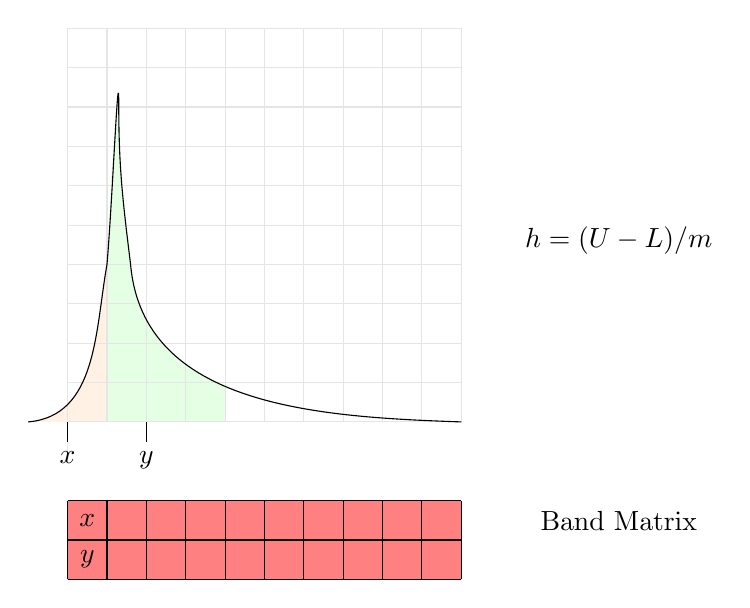
\begin{tikzpicture}

        \draw[gray!20] (0,-.5) -- (0,5);
        \draw[gray!20] (-.5,0) -- (5,0);
        \fill[fill=orange!10] (-.5,0) to [out=5,in=-100] (.5,2) to [out=85,in=90] (.5,0);
        \fill[fill=green!10] (.5,2) to [out=85,in=-100] (0.65,4) to [out=-90,in=97] (.8,2) to [out=-85,in=158] (2,.45) -- (2,0) -- (.5,0);

        \draw[gray!20] (0,0) grid[step=.5] (5,5);

        \draw [>=stealth] (-.5,0) to [out=5,in=-100] (.5,2) to [out=85,in=90] (0.65,4) to [out=-90,in=97] (.8,2) to [out=-85,in=178] (5,0);
        \fill[red!50] (0, -2) -- (5,-2) -- (5, -1) -- (0,-1);
        \draw (0,-2) grid[step=.5] (5,-1);
        \draw(7,-1.5) node[above] {Band Matrix};
        \draw(7, 2) node[above] {$h = (U-L)/m$};

        \draw(.25,-1.25) node {$x$};
        \draw(.25,-1.75) node {$y$};


        \draw (0,-.25) -- (0,0);
        \draw (1,-.25) -- (1,0);
        % \draw (2,-.25) -- (2,5);
        \draw(0,-.25) node[below] {$x$};
        \draw(1,-.25) node[below] {$y$};
        % \draw(2,-.25) node[below] {$N_{int}$};


\end{tikzpicture}


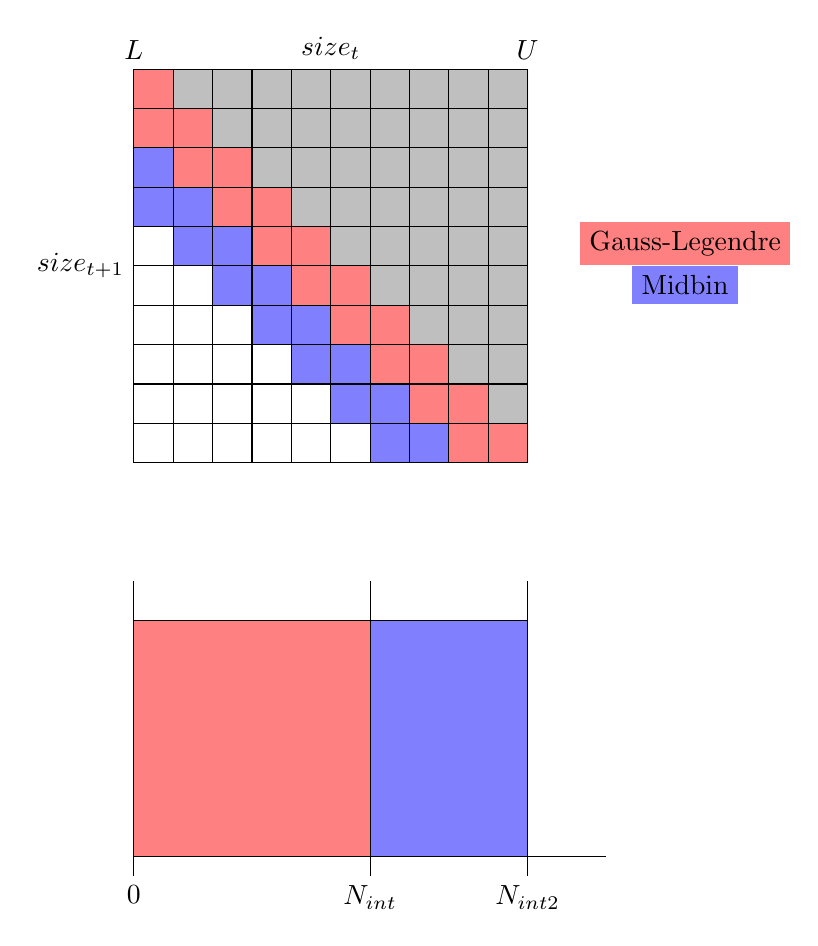
\begin{tikzpicture}
        \foreach \i in {3,2.5,...,0}{
                        {\fill[blue!50] (\i, 5-\i-2) -- (5,5-\i-2) -- (5,5) -- (\i,5);}
                }
        \foreach \i in {4,3.5,...,0}{
                        {\fill[red!50] (\i, 5-\i-1) -- (5,5-\i-1) -- (5,5) -- (\i,5);}
                }
        \foreach \i in {5,4.5,...,0.5}{
                        {\fill[gray!50] (\i, 5-\i) -- (5,5-\i) -- (5,5) -- (\i,5);}
                }

        \draw (0,0) grid[step=.5] (5,5);
        \draw (2.5,5) node[above]{$size_t$} ;
        \draw (0,2.5) node[left]{$size_{t+1}$} ;
        \draw(0,5) node[above] {$L$};
        \draw(5,5) node[above] {$U$};

        \draw(7,2.5) node[fill=red!50,above] {Gauss-Legendre};
        \draw(7,2.5) node[fill=blue!50,below] {Midbin};

        \begin{scope}[shift={(0,-5)}]
                \fill[red!50,draw=black] (0,0) -- (0,3) -- (3,3) -- (3,0);
                \fill[blue!50,draw=black] (3,0) -- (3,3) -- (5,3) -- (5,0);
                \draw (5,-.25) -- (5,3.5);
                \draw (0,-.25) -- (0,3.5);
                \draw (3,-.25) -- (3,3.5);
                \draw (5,-.25) -- (5,3.5);
                \draw (0,0) -- (6,0);
                \draw(0,-.25) node[below] {$0$};
                \draw(3,-.25) node[below] {$N_{int}$};
                \draw(5,-.25) node[below] {$N_{int2}$};
        \end{scope}


\end{tikzpicture}

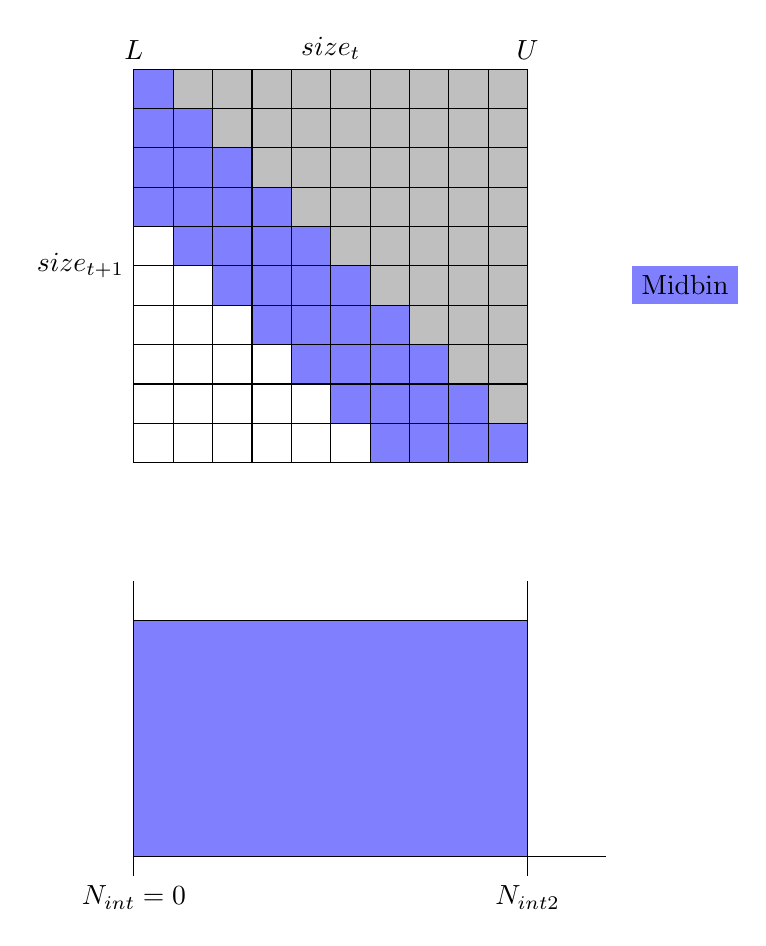
\begin{tikzpicture}
        \foreach \i in {3,2.5,...,0}{
                        {\fill[blue!50] (\i, 5-\i-2) -- (5,5-\i-2) -- (5,5) -- (\i,5);}
                }
        \foreach \i in {5,4.5,...,0.5}{
                        {\fill[gray!50] (\i, 5-\i) -- (5,5-\i) -- (5,5) -- (\i,5);}
                }

        \draw (0,0) grid[step=.5] (5,5);
        \draw (2.5,5) node[above]{$size_t$} ;
        \draw (0,2.5) node[left]{$size_{t+1}$} ;
        \draw(0,5) node[above] {$L$};
        \draw(5,5) node[above] {$U$};

        \draw(7,2.5) node[fill=blue!50,below] {Midbin};

        \begin{scope}[shift={(0,-5)}]
                \fill[blue!50,draw=black] (0,0) -- (0,3) -- (5,3) -- (5,0);
                \draw (5,-.25) -- (5,3.5);
                \draw (0,-.25) -- (0,3.5);
                \draw (5,-.25) -- (5,3.5);
                \draw (0,0) -- (6,0);
                \draw(0,-.25) node[below] {$N_{int} = 0$};
                \draw(5,-.25) node[below] {$N_{int2}$};
        \end{scope}



\end{tikzpicture}

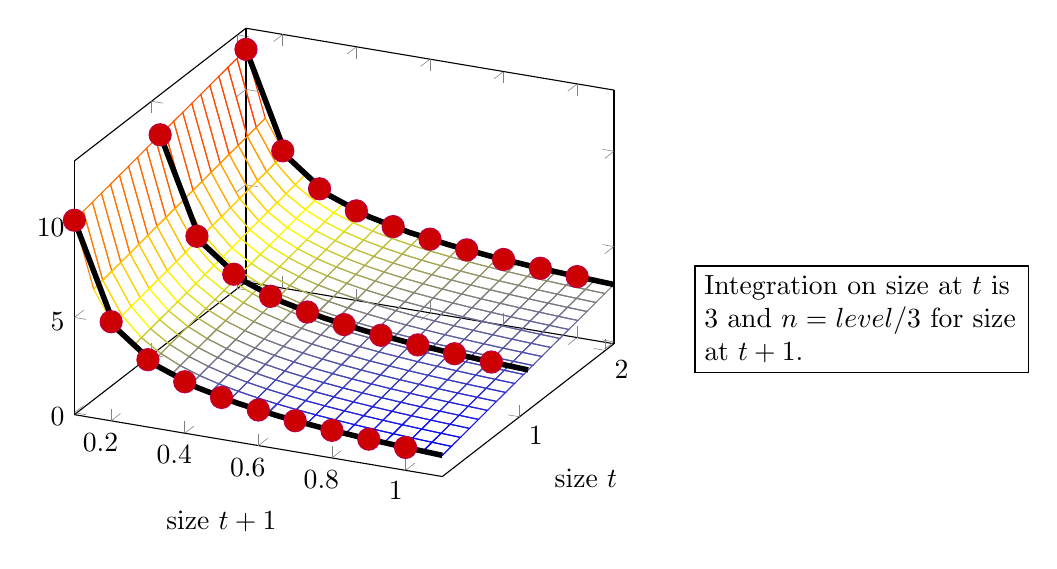
\begin{tikzpicture}
        \begin{axis}[xlabel={size $t+1$}, ylabel={size $t$}]

                \addplot3[mesh, shader=interp, samples=20, domain=0.1:1.1, domain y = 0.1:2.1] {1 /x + y};
                \addplot3+ [domain=0.1:1, domain y=0.1:2.1,samples=10,samples y=3, color = purple,
                        only marks,mark=*,mark size=4pt] {1 /x + y};
                \foreach \l in {0.1,1.1,2.1}{
                                \addplot3[domain=0.1:1.1, domain y= 0.1:2.1, samples=10,samples y=0, line width=2pt]
                                (x,\l,1/x + \l);
                        }

        \end{axis}

        \begin{scope}[shift={(10,0)}]
                \node[draw,text width=4cm] at (0,2) {Integration on size at $t$ is $3$ and $n=level/3$ for size at $t+1$.};
        \end{scope}

\end{tikzpicture}

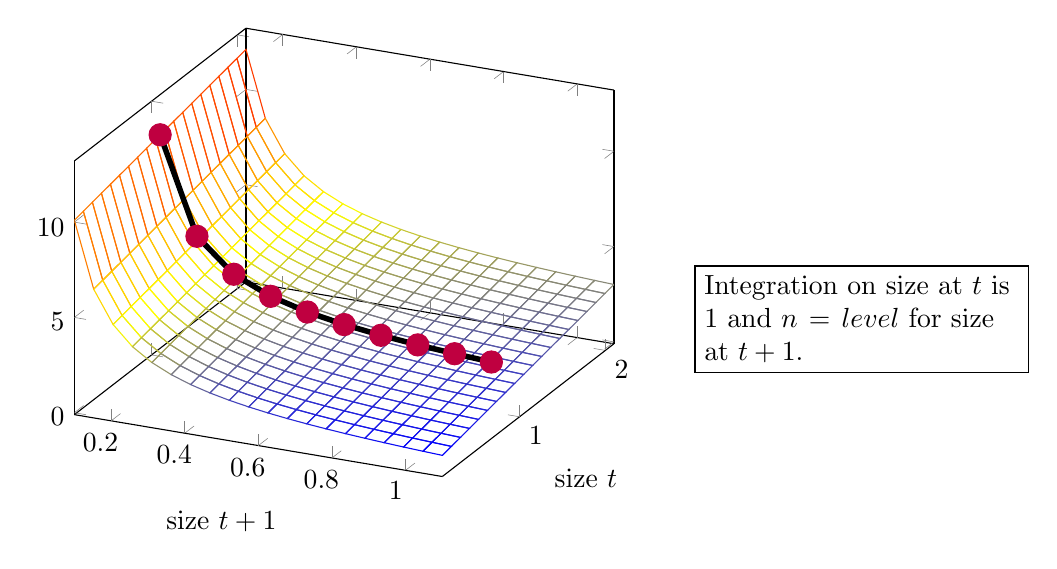
\begin{tikzpicture}
        \begin{axis}[xlabel={size $t+1$}, ylabel={size $t$}]

                \addplot3[mesh, shader=interp, samples=20, domain=0.1:1.1, domain y = 0.1:2.1] {1 /x + y};
                \addplot3[domain=0.1:1, domain y= 0.1:2.1, samples=10,samples y=0, 
                        only marks,mark=*,mark size=4pt, color = purple]
                        (x,1.1,1/x + 1.1);
                \addplot3[domain=0.1:1, domain y= 0.1:2.1, samples=10,samples y=0, line width=2pt]
                        (x,1.1,1/x + 1.1);
                

        \end{axis}

        \begin{scope}[shift={(10,0)}]
                \node[draw,text width=4cm] at (0,2) {Integration on size at $t$ is $1$ and $n=level$ for size at $t+1$.};
        \end{scope}

\end{tikzpicture}


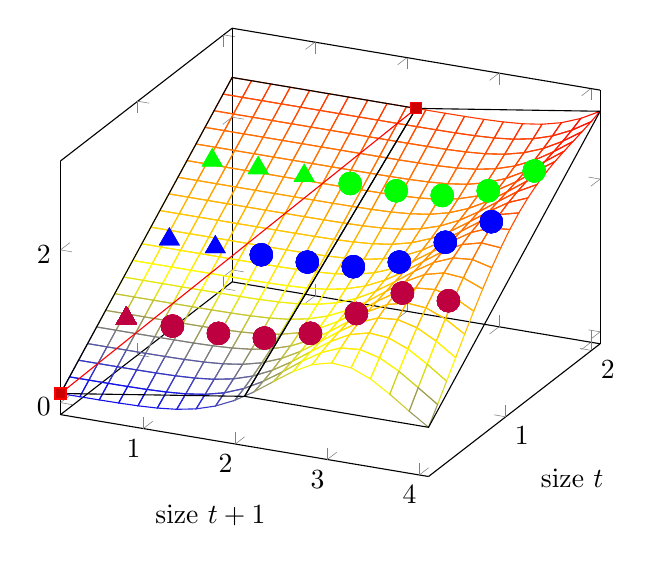
\begin{tikzpicture}[declare function = {f(\x, \y) = exp(-(\x-(\y+3))^2)+\y*1.2;}]
        \begin{axis}[xlabel={size $t+1$}, ylabel={size $t$}]

                \addplot3[mesh, shader=interp, samples=20, domain=0.1:4.1, domain y = 0.1:2.1] {f(x, y)};
                \addplot3 table [z expr = exp(-(x-(y+3))^2) + y*1.2, x = col1,  y = col2, color = black] 
                        {
                        col1 col2
                        0.1 0.1
                        2.1  2.1
                        };
                \addplot3[mesh, shader=interp,samples=3,samples y = 2,domain=0.1:4.1,domain y = 0.1:2.1, color = black] 
                {f(x, y)};

                \addplot3[mark=triangle*,mark size=4pt, color = purple]
                        (0.35,0.6, {exp(-(0.35-(0.6+3))^2) + 0.6 * 1.2});
                \addplot3[domain=0.35:0.85, samples=2, only marks,mark=triangle*,mark size=4pt, color = blue]
                        (x,1.1, {exp(-(x-(1.1+3))^2) + 1.1 * 1.2});
                \addplot3[domain=0.35:1.35, samples=3, only marks,mark=triangle*,mark size=4pt, color = green]
                        (x,1.6,{exp(-(x-(1.6+3))^2) + 1.6 * 1.2});

                \addplot3[domain=0.85:3.85, samples=7, only marks,mark=*,mark size=4pt, color = purple]
                        (x,0.6,{exp(-(x-(0.6+3))^2) + 0.6 * 1.2});
                \addplot3[domain=1.35:3.85, samples=6, only marks,mark=*,mark size=4pt, color = blue]
                        (x,1.1, {exp(-(x-(1.1+3))^2) + 1.1 * 1.2});
                \addplot3[domain=1.85:3.85, samples=5, only marks,mark=*,mark size=4pt, color = green]
                        (x,1.6, {exp(-(x-(1.6+3))^2) + 1.6 * 1.2} );


                % \addplot3[mesh, shader=interp, samples=20, domain=2.1:6.1, domain y = 2.1:4.1] {f(x, y)};


        \end{axis}
\end{tikzpicture}


\begin{tikzpicture}[scale = 0.9]
        \matrix (m)
          [
            matrix of nodes,
            nodes in empty cells,
            column sep      = 3em,
            row sep         = 5ex,
            column 1/.style = { nodes = { empty } },
            column 2/.style = { nodes = { empty } },
            column 3/.style = { nodes = { empty } },
            column 4/.style = { nodes = { empty } },
          ]
          {
              &  &  &  \\
              File.txt &  & File.txt & \com \\  % \textit{7f21c09}
              File1.txt &  & File.txt & \com \\ % \textit{d39ac60}
              File2.txt &  & File.txt & \com \\ % \textit{c78c64d}
              File\_final.txt &  & File.txt & \com \\ % \textit{cbdac1e}
          };
          \node[fit=(m-1-1)(m-1-1)]{Saving copies};
          \node[fit=(m-1-3)(m-1-4)]{Git workflow};
      
        \foreach \i/\j in {2/3,3/4,4/5} {
          \draw [arrow] (m-\i-4) -- (m-\j-4);
          \draw [arrow] (m-\i-3) -- (m-\i-4);
          \pic at (m-\i-2) {file};
        }
        \draw [arrow] (m-5-3) -- (m-5-4);
        \pic at (m-5-2) {file};
        
      \end{tikzpicture}


\end{document}